  %%%%%%%%%%%%%%%%%%%%%%%%%%%%%%%%%%%%%%%%%%
  %%                                      %%
  %%AQUI SÃO INSERIDOS OS PACOTES DO LATEX%%
  %%                                      %%
  %%%%%%%%%%%%%%%%%%%%%%%%%%%%%%%%%%%%%%%%%%
  
\documentclass[a4paper, 12pt]{article}
\usepackage[top=3cm, botton=2cm, left=3cm, right=2cm]{geometry}
\usepackage[utf8]{inputenc}
\usepackage{float}
\usepackage{graphicx}
\usepackage[brazilian, english]{babel}
\usepackage{fancyhdr}
\usepackage{amsmath, amsfonts, amssymb}
\usepackage{xcolor}
\usepackage{xwatermark}
\usepackage{epigraph}
\usepackage{tabularx}
\usepackage{abstract}
\usepackage{subfig}
\usepackage{emptypage}
%%%%%%%%%%%%%%%%%%%%%%%%%%%%%%%%%%%%%%%%%%%%%%%%%%%%
%%  USADO PARA PRODUZIRMOS UMA CAPA PARA O ARTIGO %%
%%%%%%%%%%%%%%%%%%%%%%%%%%%%%%%%%%%%%%%%%%%%%%%%%%%%
                                               
%\documentclass{ufpethesis}
%\title{Aqui é o título}
%\author{Nome do autor}
%\date{2015}




%% INÍNCIO DO ARTIGO %%
\newwatermark[allpages]{
\includegraphics[scale=0.7]{backgroud-logo-rm}}
\begin{document}

\graphicspath{{imagens/}{referencias/}{logo/}}  %% Referenciando subpastas no arquivo %%
\pagestyle{fancy} 
%% ESPAÇO DIDICADO À AGRADECIMENTOS, RESUMO E ABSTRACT %%

\begin{titlepage}
\centering
\begin{Large}
 \underline{\textbf{PORTFÓLIO PRESTAÇÃO DE SERVIÇOS}}
 \end{Large} 
\begin{center}
\begin{figure}[!htbp]
\centering

\includegraphics[scale=0.4,opacity=0.8]{logo-completo-rm-facilities}
\end{figure}
\end{center}
\begin{huge}
\underline{Produtos}
\end{huge} \vspace{2cm}

\begin{LARGE}
\underline{\textbf{ MÃO DE OBRA}} 
\end{LARGE}
\vspace{1cm}

\begin{LARGE}
\underline{\textbf{ QUALIFICADA}}
\end{LARGE}
\vspace{4cm}

\centering
CONHEÇA-NOS MELHOR COMEÇANDO POR
\textbf{AQUI!}

\vspace{2.6cm}
\begin{figure}
\centering

\includegraphics[scale=0.5]{endereço-portifólio}
\end{figure}

\end{center}

\end{titlepage}

%\begin{titlepage}

%\selectlanguage{english}
%\begin{abstract}
 %Text in English
%\end{abstract}
%\begin{footnotesize}
%\textbf{keywords:} \textit{key words}
%\end{footnotesize}
%\newpage

%\begin{center}
%\textbf{Agradecimentos}
%\end{center}

%Agradecimentos aqui!

%\end{titlepage}

%% EPÍGRAFE DO ARTIGO %%
\begin{titlepage}

   \epigraph{\textit{"A caridade é o processo de somar alegrias, diminuir males, multiplicar esperanças e dividir a felicidade para que a Terra se realize na condição do esperado Reino de Deus."}}{Emmanuel} \newpage

\end{titlepage}
\newpage



%%  SUMÁRIO  %%
%\selectlanguage{brazilian}
%\tableofcontents \newpage  %% ESTE COMANDO ABILITA O SUMÁRIO NO ARTIGO  %% 

%%  LISTA DE FIGURAS E TABELAS %%

%\listoffigures
%\listoftables
%\newpage

%  Comando para a insersão da capa neste ponto do artigo  $$
%\maketitle

%% LOGOTIPO NO CABEÇALHO %%
\pagestyle{fancy} 
\lhead{
\includegraphics[width=4cm]{logo-completo-rm-facilities}}
\rhead{PORTFÓLIO PRESTAÇÃO DE SERVIÇOS}
%% NOTAS DE RODAPÉ %%
\rfoot{\begin{small}rmfacilities.com.br\end{small}}
\lfoot{}



%%%%%%%%%%%%%%%%%%%%%%%%%%%%%%%%%%
%%%                            %%%
%%% INÍCIO DO CORPO DO ARTIGO, %%%
%%%                            %%%
%%%%%%%%%%%%%%%%%%%%%%%%%%%%%%%%%%


\section*{}
%\maketitle
%% Inclusão de Figuras %%


%% inclusão de SubFiguras %%

\begin{figure}[!htb]
\centering
\subfloat[Aline]{

\includegraphics[height=4cm]{1}
\label{figdroopy}
}
\quad %espaco separador
\subfloat[Mel]{

\includegraphics[height=4cm]{2}
\label{figsnoop}
}
\caption{Minhas Vidas}
\label{fig01}
\end{figure}

\begin{figure}[!htb]
\centering
\subfloat[Aline]{

\includegraphics[height=4cm]{3}
\label{figdroopy}
}
\quad %espaco separador
\subfloat[Mel]{
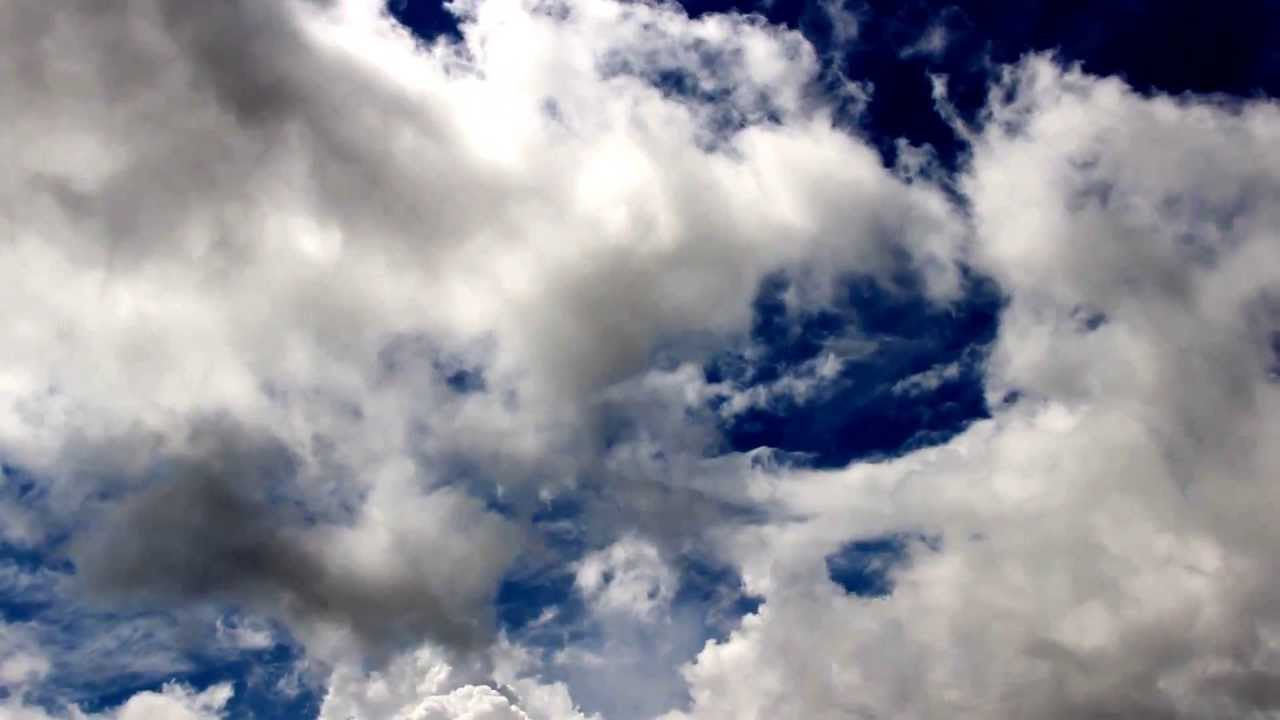
\includegraphics[height=4cm]{4}
\label{figsnoop}
}
\caption{Minhas Vidas}
\label{fig01}
\end{figure}


\begin{figure}[!htb]
\centering
\subfloat[Aline]{
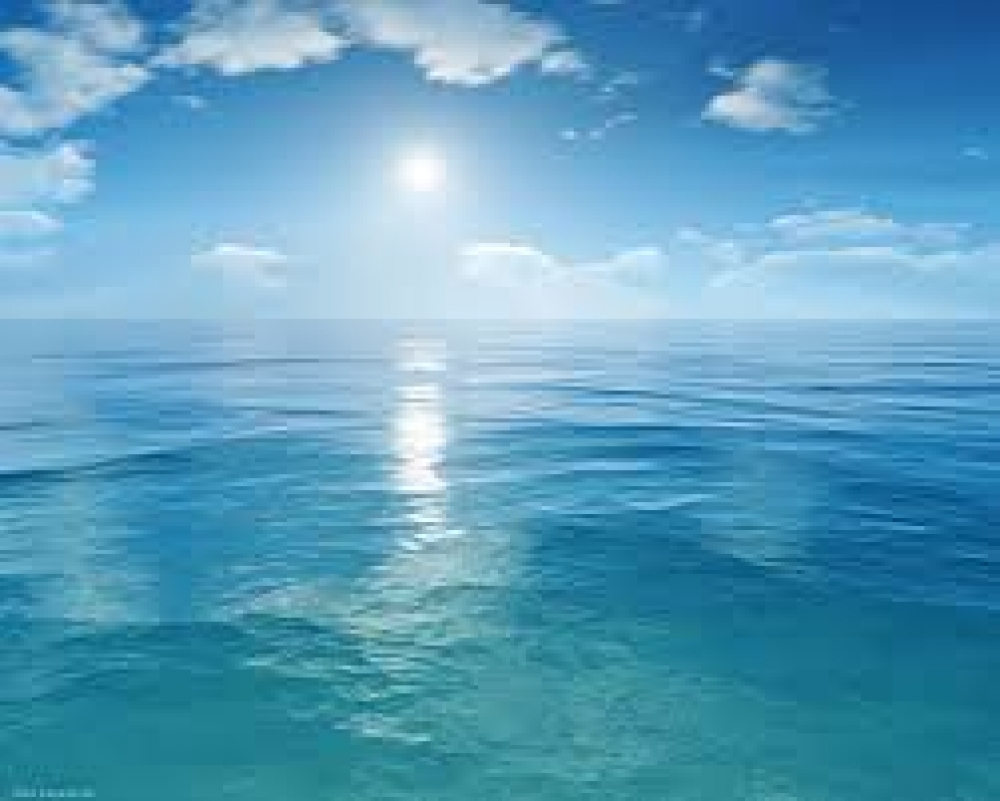
\includegraphics[height=4cm]{5}
\label{figdroopy}
}
\quad %espaco separador
\subfloat[Mel]{
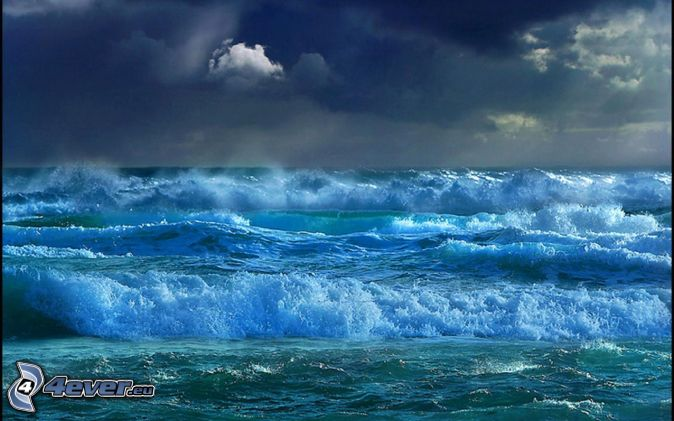
\includegraphics[height=4cm]{6}
\label{figsnoop}
}
\caption{Minhas Vidas}
\label{fig01}
\end{figure}



\begin{figure}[!htb]
\centering
\subfloat[Aline]{
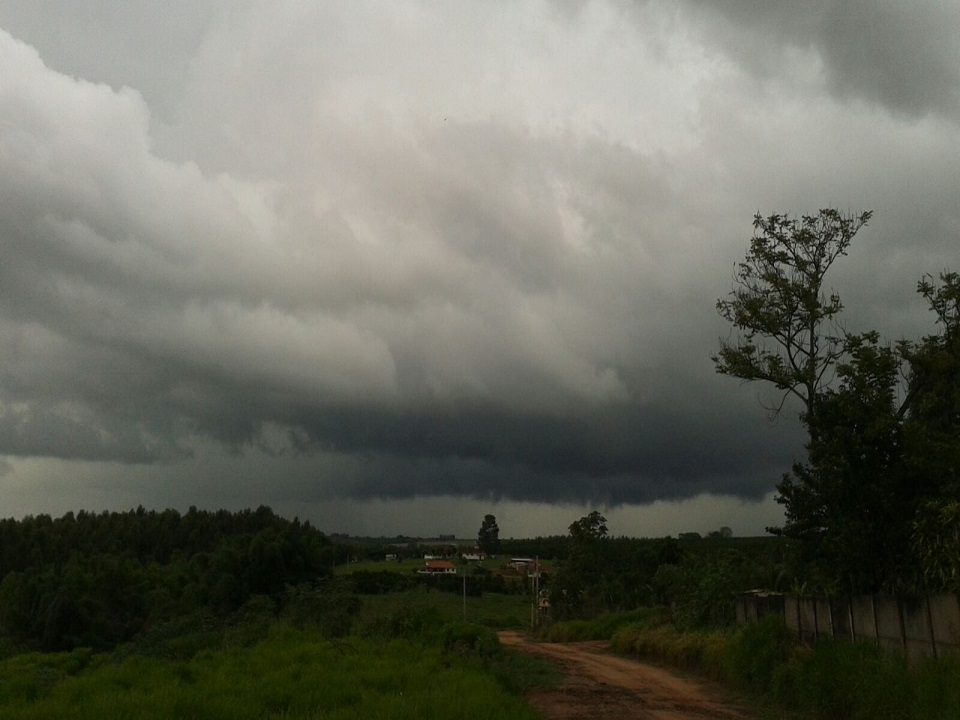
\includegraphics[height=4cm]{7}
\label{figdroopy}
}
\quad %espaco separador
\subfloat[Mel]{
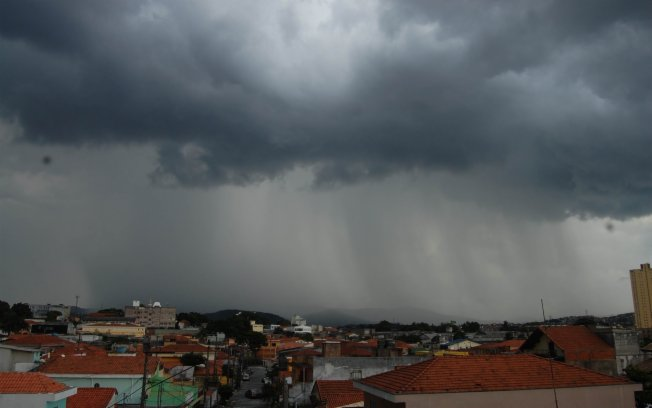
\includegraphics[height=4cm]{8}
\label{figsnoop}
}
\caption{Minhas Vidas}
\label{fig01}
\end{figure}

\begin{figure}[!htb]
\centering
\subfloat[Aline]{
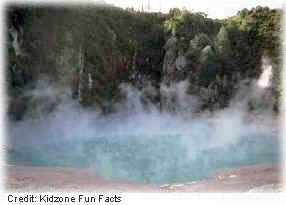
\includegraphics[height=4cm]{9}
\label{figdroopy}
}
\quad %espaco separador
\subfloat[Mel]{

\includegraphics[height=4cm]{1}
\label{figsnoop}
}
\caption{Minhas Vidas}
\label{fig01}
\end{figure}






 

%%% REFERENCIAS BIBLIOGRAFICAS %% 
\newpage
\bibliographystyle{plain}
\addcontentsline{toc}{section}{REFERÊNCIAS} 
\bibliography{referencias/biblio.bib}

\cite{evangelho}
\cite{le}


\end{document}
